%----------------------------------------------------------------------------------------
%	PACKAGES AND OTHER DOCUMENT CONFIGURATIONS
%----------------------------------------------------------------------------------------

\documentclass{article}

\usepackage[utf8]{inputenc}
\usepackage{amssymb}
\usepackage{amsmath}
\usepackage{float}
\usepackage{latexsym}
\usepackage{subcaption}
\usepackage{gensymb}
\usepackage{caption}
\usepackage{fancyhdr} % Required for custom headers
\usepackage{lastpage} % Required to determine the last page for the footer
\usepackage{extramarks} % Required for headers and footers
\usepackage[usenames,dvipsnames]{color} % Required for custom colors
\usepackage{graphicx} % Required to insert images
\usepackage{listings} % Required for insertion of code
\usepackage{courier} % Required for the courier font
\usepackage{lipsum}
\usepackage{tabularx}
\usepackage{color}

\definecolor{mygreen}{rgb}{0,0.6,0}
\definecolor{mygray}{rgb}{0.5,0.5,0.5}
\definecolor{mymauve}{rgb}{0.58,0,0.82}

\lstset{
  backgroundcolor=\color{white},   % you must add \usepackage{color} or \usepackage{xcolor}
  breaklines=true,                 % sets automatic line breaking
  captionpos=b,                    % sets the caption-position to bottom
  commentstyle=\color{mygreen},    % comment style
  escapeinside={\%*}{*)},          % if you want to add LaTeX within your code
  extendedchars=true,              % lets you use non-ASCII characters; for 8-bits encodings only, does not work with UTF-8
  frame=single,	                   % adds a frame around the code
  keepspaces=true,                 % keeps spaces in text, useful for keeping indentation of code (possibly needs columns=flexible)
  keywordstyle=\color{blue},       % keyword style
  language=Octave,                 % the language of the code
  otherkeywords={*,...},           % if you want to add more keywords to the set
  numbers=left,                    % where to put the line-numbers; possible values are (none, left, right)
  numbersep=5pt,                   % how far the line-numbers are from the code
  numberstyle=\tiny\color{mygray}, % the style that is used for the line-numbers
  rulecolor=\color{black},         % if not set, the frame-color may be changed on line-breaks within not-black text (e.g. comments (green here))
  showspaces=false,                % show spaces everywhere adding particular underscores; it overrides 'showstringspaces'
  showstringspaces=false,          % underline spaces within strings only
  showtabs=false,                  % show tabs within strings adding particular underscores
  stepnumber=2,                    % the step between two line-numbers. If it's 1, each line will be numbered
  stringstyle=\color{mymauve},     % string literal style
  tabsize=2,	                   % sets default tabsize to 2 spaces
  title=\lstname                   % show the filename of files included with \lstinputlisting; also try caption instead of title
}

\topmargin=-0.45in
\evensidemargin=0in
\oddsidemargin=0in
\textwidth=6.5in
\textheight=9.0in
\headsep=0.25in
\linespread{1.1} % Line spacing

\pagestyle{fancy}
\lhead{ATML - Assignment 1} % Top left header
\chead{}
\lfoot{\lastxmark} % Bottom left footer
\cfoot{} % Bottom center footer
\rfoot{Page\ \thepage} % Bottom right footer
\renewcommand\headrulewidth{0.4pt} % Size of the header rule
\renewcommand\footrulewidth{0.4pt} % Size of the footer rule
\setlength\parindent{16pt} % Removes all indentation from paragraphs
\setcounter{secnumdepth}{0} % Removes default section numbers
\title{
\vspace{1in}
\textmd{\textbf{Advanced Topics in Machine Learning - Assignment 1}} \\
\author{Christoffer Thrysøe - dfv107}
}
%%%%%%%%%%%%%%%%%%%%%%%%%%%%%%%%%%%%%%%%%%%%%%%%%%%%%%%%%%%%%%%%%%%%%%%%
\begin{document}
\maketitle
\pagenumbering{arabic}
\section{1 Numerical comparison of kl inequality with its relaxations
and with Hoeffding’s inequality}
\subsection{1}
\subsubsection*{A}
Hoeffding’s bound on p is as followed:
\begin{equation*}
P \left\lbrace p \leq \hat{p} + \sqrt{ \dfrac{ln \frac{1}{\delta}}{2n}} \right\rbrace > 1 - \delta
\end{equation*}
\subsubsection{B}
By theorem 2.14 from Yevgeny's lecture notes, we have the following bound on the kl-inequality:
\begin{equation}
\label{eq:214}
P \left\lbrace \text{kl}(\hat{p} || p) \geq \epsilon \right\rbrace \leq (n+1) e^{-n\epsilon}
\end{equation}
Setting the right hand side of \eqref{eq:214} equal to $\delta$, we get the following bound on $\text{kl}(\hat{p}||p)$, with probability greater than $1- \delta$:
\begin{equation}
\label{eq:z}
\text{kl}(\hat{p} || p) \leq \dfrac{ln \frac{n+1}{\delta}}{n}
\end{equation}
We can derive a bound for $p$ by taking the upper inverse of $\text{kl}(\hat{p}||p)$, which is defined as:
\begin{equation}
\text{kl}^{-1^+}(\hat{p},z) = \text{max} \left\lbrace p: \text{kl}(\hat{p}||p) \leq z \right\rbrace
\end{equation}
and if $\text{kl}(\hat{p}||p) \leq z$ then $p \leq \text{kl}^{-1^+}(\hat{p},z)$. If we denote the right hand side of \eqref{eq:z} by $z$ and exchange the definition of $\text{kl}(\hat{p}||p)$ with definition 2.11 from Yevgeny's lecture notes, we get the following bound for $p$:
\begin{align*}
P \left\lbrace p \leq \text{max} \left\lbrace p: p \text{ ln} \frac{\hat{p}}{p} + (1-\hat{p}) \text{ ln } \dfrac{1-\hat{p}}{p} \leq \dfrac{ln \frac{n+1}{\delta}}{n} \right\rbrace \right \rbrace > 1 - \delta
\end{align*}
Note that for the plot, the above bound on $p$ was done using the provided matlab function \texttt{ysidkl.m}, which computes the upper inverse of the kl inequality using a binary search.
\subsubsection{C}
Pinsker's relaxation of the kl inequality gives the following bound on p:
\begin{align*}
|p - \hat{p}| &\leq \sqrt{\dfrac{\text{kl}(\hat{p}||p)}{2}} \leq \sqrt{\dfrac{ln \frac{n+1}{\delta}}{2n}} \\
p &\leq \hat{p} + \sqrt{\dfrac{\text{kl}(\hat{p}||p)}{2}} \leq \hat{p} + \sqrt{\dfrac{ln \frac{n+1}{\delta}}{2n}}
\end{align*}
Thus we have the following bound on $p$:
\begin{equation}
P \left\lbrace p \leq \hat{p} + \sqrt{\dfrac{ln \frac{n+1}{\delta}}{2n}} \right\rbrace > 1 - \delta
\end{equation}

\subsubsection{D}
The refined Pinsker's relaxation of the kl inequality gives the following bound on $p$:
\begin{equation}
P \left\lbrace p \leq \hat{p} + \sqrt{\dfrac{2 \hat{p} \text{ } ln \frac{n+1}{\delta}}{n}} + \dfrac{2 ln \frac{n+1}{\delta}}{n} \right\rbrace > 1 - \delta
\end{equation}
\subsection{2}
Figure \ref{fig:1} shows the four aforementioned upper bounds on p, plotted as a function of $\hat{p}$, these bounds will be discussed in section 4 of the assignment.
\begin{figure}[H]
  \centering
  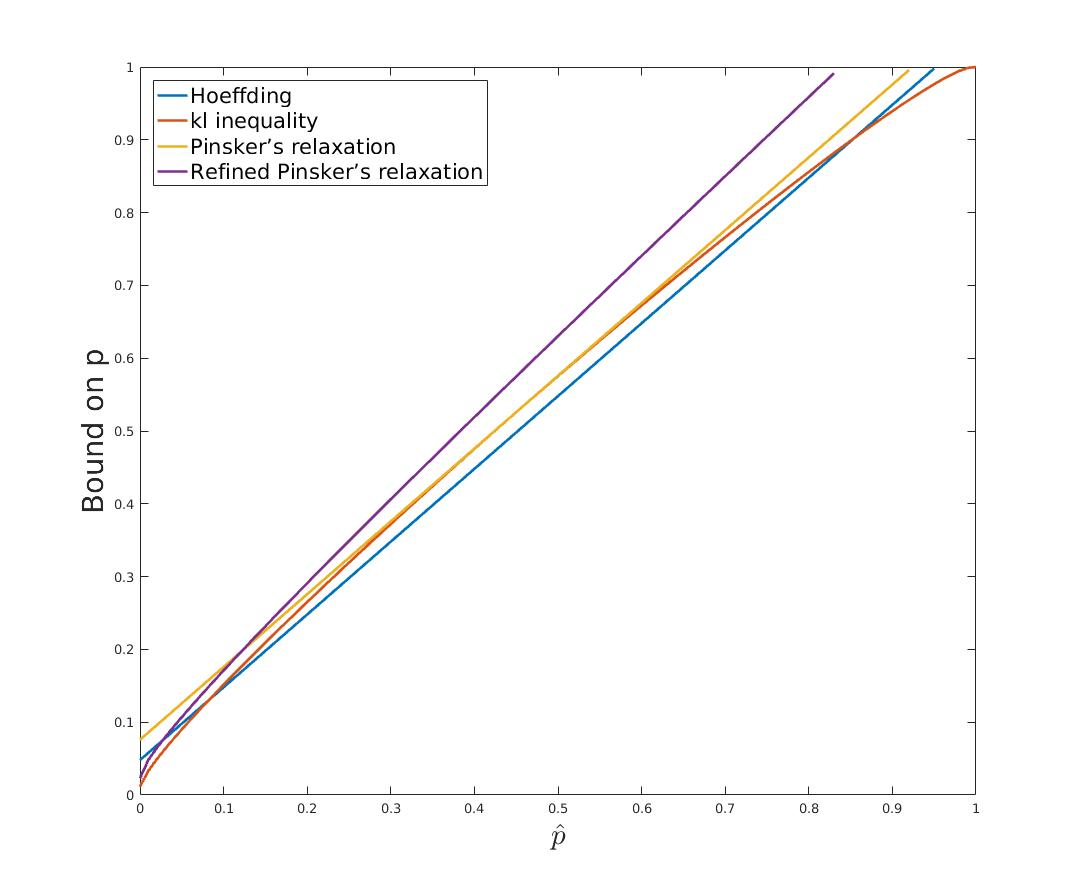
\includegraphics[width=17cm]{fig/5.jpg}
  \caption{\footnotesize The upper bound on $p$ for the four bounds, plotted as a function of $\hat{p}$}
    \label{fig:1}
\end{figure}
\subsection{3}
Hoeffding’s lower bound on $p$ is given by:
%\begin{equation*}
%P \left\lbrace p > \hat{p}_n + \sqrt{ \dfrac{ln \frac{1}{\delta}}{2n}} %\right\rbrace \leq \delta
%\end{equation*}
\begin{equation*}
P \left\lbrace p > \hat{p} - \sqrt{ \dfrac{ln \frac{1}{\delta}}{2n}} \right\rbrace > 1-\delta
\end{equation*}
The kl inequality lower bound on $p$ is achieved by taking the lower inverse of the kl inequality, which is defined as:
\begin{equation}
kl^{-1^-}(\hat{p},z) = \text{min} \lbrace p: \text{kl}(\hat{p} || p) \leq z \rbrace
\end{equation}
The lower bound can be stated as followed:
\begin{align*}
&P \left\lbrace p > \text{min} \lbrace p: \text{kl}(\hat{p} || p) \leq z \rbrace \right \rbrace > 1-\delta  \\
=&P \left\lbrace p > \text{min} \left\lbrace p : p \text{ ln} \frac{\hat{p}}{p} + (1-\hat{p}) \text{ ln } \dfrac{1-\hat{p}}{p} \leq \dfrac{ln \frac{n+1}{\delta}}{n} \right \rbrace \right\rbrace > 1- \delta
\end{align*}
The above minimization problem was solved using a binary search approach adopted from the existing provided matlab function. The program (\texttt{klmin.m}) simply evaluates if the condition $\text{kl}(\hat{p}||p) \leq z$ is satisfied and if so reduces $p$. If the condition is not met, p is changed to increase $\text{kl}(\hat{p}||p)$. Figure \ref{fig:2} shows the two lower bounds on $p$, plotted as a function of $\hat{p}$.
\begin{figure}[H]
  \centering
  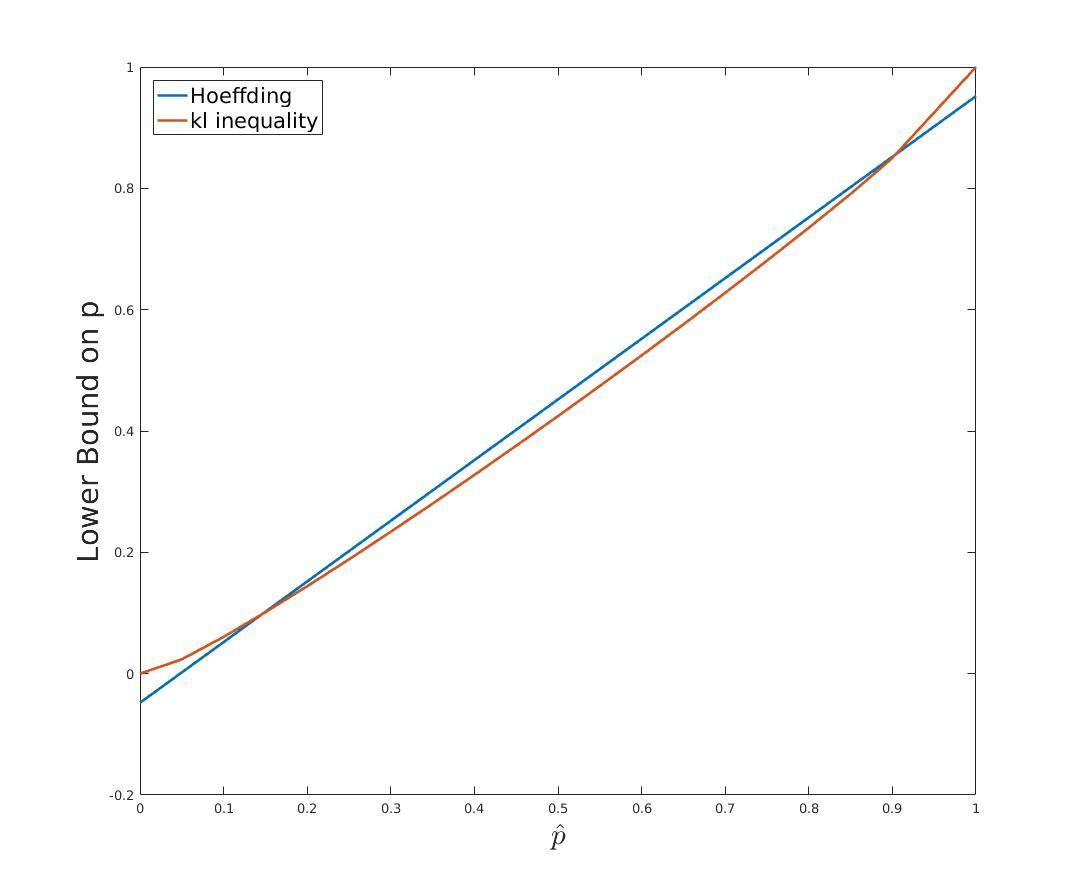
\includegraphics[width=17cm]{fig/3.jpg}
  \caption{\footnotesize The Hoeffding’s and kl inequality lower bound, plotted as a function of $\hat{p}$}
    \label{fig:2}
\end{figure}
\subsection{4}
Comparing Hoeffding’s upper bound with Pinsker's relaxation bound in figure \ref{fig:1}, it is clear that Hoeffding’s bound is tighter due to the $n+1$ term in Pinkser's relaxation. The refined Pinkser's relaxation provides a tighter bound than Hoeffding’s when $\hat{p}$ is low, providing a high confidence in the bound, which is due to the second term dominating the first, whereas for larger values of $\hat{p}$, the first term grows large, resulting in a looser bound. As expected, the kl inequality bound is tighter than it's relaxations. The kl inequality bound provides a significantly tighter bound for $\hat{p} \in [0,0.1]$ and $\hat{p} \in [0.9,1]$ thus a greater confidence in the bound for small and large empirical errors. Hoeffding's bound is tighter than the kl inequality bound for $\hat{p} \in [0.2,0.8]$.\\ \\
The lower bounds on $p$, shown in figure \ref{fig:2}, are very similar to their correspondent upper bounds in the sense that the kl lower bound provides a tighter bound for $\hat{p} \in [0,0.1]$ and $\hat{p} \in [0.9,1]$ whereas Hoeffding's lower bound provide a stronger bound for $p\in [0.2,0.8]$.
\section{2 Occam’s razor with kl inequality}
We wish to prove that for all $h \in \mathcal{H}$:
\begin{equation}
\label{eq:proove}
P \left\lbrace \text{kl}(\hat{L}(h,S) || L(h)) \leq \dfrac{ln  \frac{n+1}{p(h) \delta} }{n} \right\rbrace > 1 - \delta
\end{equation}
% lhat bernuilli
where
$$
\sum\limits_{h \in \mathcal{H}} p(h) \leq 1
$$
First we use theorem 2.14 from Yevgeny's lecture notes, which states:
\begin{equation}
\label{eq:theorem14}
P\left\lbrace \text{kl}(\hat{p} || p) \geq \epsilon \right\rbrace \leq (n+1)e^{-n\epsilon}
\end{equation}
We can use this theorem as $L(h)$ is our bias and $\hat{L}(h,s)$ is our empirical bias.\\
replacing $\epsilon$ with the desired bound:
$$
\epsilon = \dfrac{ln  \frac{n+1}{p(h) \delta} }{n}
$$
in \eqref{eq:theorem14} we get:
\begin{equation}
\label{eq:lastineq}
P\left\lbrace \text{kl}(\hat{L}(h,S) || L(h)) \geq \dfrac{ln  \frac{n+1}{p(h) \delta} }{n} \right\rbrace \leq (n+1)e^{-n\dfrac{ln  \frac{n+1}{p(h) \delta} }{n}}
\end{equation}
% = p(h) \delta
By utilizing that $e^{log(x)} = x$ we can further expand the right hand side of the last inequality of \eqref{eq:lastineq} to the following:
\begin{align*}
(n+1)e^{-n\dfrac{ln  \frac{n+1}{p(h) \delta} }{n}}
&= (n+1)\dfrac{1}{\left(\frac{n+1}{p(h) \delta}\right)} \\
&=  p(h) \delta
\end{align*}
We note that we are able to multiply $p(h)$ and $\delta$ because $p(h)$ is independent of the sample $S$. This is necessary because otherwise the probability of the bound not holding: $\delta$ would be dependent on $p(h)$ and we could therefore not multiply the dependent events, therefore $p(h)$ has to be chosen before we observe the sample $S$. \\
To show it for all $h \in \mathcal{H}$ we take the union bound over all hypothesis:
\begin{align*}
P\left\lbrace \exists h \in \mathcal{H} : \text{kl}(\hat{L}(h,S) || L(h)) \geq \dfrac{ln  \frac{n+1}{p(h) \delta} }{n} \right\rbrace
&\leq \sum\limits_{h \in \mathcal{H}} P\left\lbrace \exists h \in \mathcal{H} : \text{kl}(\hat{L}(h,S) || L(h)) \geq \dfrac{ln  \frac{n+1}{p(h) \delta} }{n} \right\rbrace \\
&\leq \sum\limits_{h \in \mathcal{H}} (n+1)e^{-n\dfrac{ln  \frac{n+1}{p(h) \delta} }{n}} \\
&= \sum\limits_{h \in \mathcal{H}} p(h) \delta \\
&\leq \delta
\end{align*}
Where the last inequality follows our definition of $p(h)$. Thus we have for all hypothesis in $\mathcal{H}$ that with probability greater than $1-\delta$:
$$
\text{kl}(\hat{L}(h,S) || L(h)) \leq \dfrac{ln  \frac{n+1}{p(h) \delta} }{n}
$$
%TODO discuss on independency of sample!
% The probability delta is independent of p(h)
% The probability bound will be dependent on p(h) as they are dependent events therefore we cannot multiply them?
\section{3 Refined Pinsker’s Lower Bound}
We wish to prove that if $\text{kl}(p||q) \leq \epsilon$ then 
\begin{equation}
\label{eq:whatweneed}
q \geq p - \sqrt{2 p \epsilon}
\end{equation}
For the proof we will prove it for $p>q$, $p<q$ and $p=q$.
\subsubsection{$\mathbf{p > q}$}
We use Corollary 2.17 from Yevgeny's lecture notes for when $p>q$ :
\begin{align}
\text{kl}(p||q) &\geq \dfrac{(p-q)^2}{2 \text{ max}\lbrace p,q \rbrace} + \dfrac{(p-q)^2}{2 \text{ max}\lbrace (1-p),(1-q)\rbrace} \\
\label{eq:thispostiv}
&= \dfrac{(p-q)^2}{2 p} + \dfrac{(p-q)^2}{2 (1-q)} \\
\label{eq:thisfollows}
&\geq \dfrac{(p-q)^2}{2p}
\end{align}
Where \eqref{eq:thisfollows} follows because the second term of the right hand side of \eqref{eq:thispostiv} is positive. Since we have the condition: $\text{kl}(p||q) \leq \epsilon$ we can write:
\begin{align}
\epsilon \geq \text{kl}(p||q) \geq \dfrac{(p-q)^2}{2p}
\end{align}
which we can derive to:
\begin{align}
\epsilon &\geq \dfrac{(p-q)^2}{2p} \Rightarrow \\
2p\epsilon &\geq (p-q)^2 \Rightarrow \\
\sqrt{2p \epsilon} &\geq p-q \Rightarrow \\
q &\geq p - \sqrt{ 2 p \epsilon}
\end{align}
which proves \eqref{eq:whatweneed} for $p>q$
\subsubsection{$\mathbf{q > p}$}
For $q>p$ we have:
\begin{align}
q&>p \Rightarrow \\
q-p &> 0 \Rightarrow \\
\label{eq:dirtytrick}
q-p + \sqrt{2 p \epsilon} &> 0 \Rightarrow \\
q &\geq p - \sqrt{2 p \epsilon}
\end{align}
Where the inequality of \eqref{eq:dirtytrick} is satisfied because $\sqrt{2 p \epsilon}$ is positive, which proves \eqref{eq:whatweneed} for $q>p$.
\subsubsection{$\mathbf{p = q}$}
If we define a new variable $t$ for which $t=p=q$, it is clear to see that \eqref{eq:whatweneed} holds:
\begin{equation}
t \geq t - \sqrt{2 t \epsilon}
\end{equation}
because $\sqrt{2 t \epsilon} \geq 0$, the inequality will hold when $p=q$. Therefore we can write:
\begin{equation}
p \geq p - \sqrt{2 p \epsilon}
\end{equation}
which proves \eqref{eq:whatweneed} for $q=p$.
\section{4 Convexity}
\subsection{1}
We wish to show that for convex functions $f(x)$ and $g(x)$ their weighted sum: $\alpha f(x) + \beta g(x)$ by two non-negative constants $\alpha$ and $\beta$ is too convex. \\
First we note that for a function $f(x)$ to be convex it must satisfy the following:
\begin{equation}
\label{eq:convexity}
f(\lambda x_1+(1-\lambda)x_2) \leq \lambda f(x_1) + (1-\lambda)f(x_2) \text{\hspace{0.5cm}     for } \lambda \in [0,1]
\end{equation}
Therefore by convexity of $f$ and $g$ we have:
\begin{align}
\label{eq:f1}
&f(\lambda x_1+(1- \lambda )x_2) \leq \lambda f(x_1) + (1- \lambda )f(x_2) \\
\label{eq:f2}
&g(\lambda x_1+(1-\lambda)x_2) \leq \lambda g(x_1) + (1- \lambda )g(x_2)
\end{align}
Combining \eqref{eq:f1} and \eqref{eq:f2} and multiplying with the non-negative constants $\alpha$ and $\beta$ we get the following:
\begin{align}
&\alpha f(\lambda x_1 + (1-\lambda) x_2) + \beta g( \lambda x_1 + (1 - \lambda) x_2)\\
&\leq \alpha ( \lambda f(x_1) + (1 - \lambda) f(x_2)) + \beta ( \lambda g (x_1) + (1 - \lambda ) g (x_2)) \\
\label{eq:finito}
&= \lambda(\alpha f(x_1) + \beta g(x_1)) + ( 1 - \lambda) (\alpha f(x_2) + \beta g(x_2)) 
\end{align}
where \eqref{eq:finito} satisfies \eqref{eq:convexity} and therefore proofs that the weighted sum of two convex functions is convex.
\subsection{2}
We wish to show that if $g(x)$ is convex and $f(x)$ is convex and increasing, then the functional composition $f  \circ g = f(g(x))$ is convex. First we note that since $g$ is convex we write:
\begin{equation}
g(\lambda x_1 + (1 - \lambda) x_2 ) \leq \lambda g(x_1) + (1- \lambda)g(x_2) 
\end{equation}
Then, we use that $f$ is increasing:
\begin{align}
f(g(\lambda x_1 + (1 - \lambda) x_2 )) &\leq f(\lambda g(x_1) + (1- \lambda)g(x_2))\\
\label{eq:compositionresult}
&\leq \lambda f(g(x)) + (1- \lambda) f(g(x_2))
\end{align}
where the last line follows that $f$ is convex. \eqref{eq:compositionresult} satisfies the rule of convexity and therefore the composition of $f$ and $g$ is convex.
\subsection{3}
Given that $f(x)$ is a convex function and $g(x)$ is an affine linear function: $g(x) = ax +b$, we wish to show that the composition $f \circ g(x) = f(ax+b)$ is convex. To show this we must prove the following:
\begin{equation}
(f \circ g) (\lambda x_1 + (1 - \lambda) x_2) \leq \lambda(f \circ g)(x_1) + (1-\lambda)(f \circ g)(x_2)
\end{equation}

\begin{align}
(f \circ g) (\lambda x_1 + (1 - \lambda) x_2) &=
f(a(\lambda x_1 + (1 - \lambda)x_2) + \lambda b + (1-\lambda)b)\\
&= f(\lambda ( ax_1 + b) + (1-\lambda)(ax_2+b) \\
\label{eq:followconv}
&\leq \lambda f(ax_1+b) + (1-\lambda) f(ax_2 +b) \\
&= \lambda (f \circ g)(x_1) + (1-\lambda) (f \circ g) (x_2)
\label{eq:affineend}
\end{align}
Where \eqref{eq:followconv} follows from $f$ being convex. \eqref{eq:affineend} gives the desired result and the proof is therefore complete.

\end{document}